\documentclass{article}
\usepackage[utf8]{inputenc}
\usepackage[spanish]{babel}
\usepackage{listings}
\usepackage{graphicx}
\graphicspath{ {images/} }
\usepackage{cite}

\begin{document}

\begin{titlepage}
    \begin{center}
        \vspace*{1cm}
            
        \Huge
        \textbf{Proyecto de investigación}
            
        \vspace{0.5cm}
        \LARGE
        Nociones de la memoria del computador
            
        \vspace{1.5cm}
            
        \textbf{Oscar Andrés Gutiérrez Rivadeneira}
            
        \vfill
            
        \vspace{0.8cm}
            
        \Large
        Despartamento de Ingeniería Electrónica y Telecomunicaciones\\
        Universidad de Antioquia\\
        Medellín\\
        Septiembre de 2020
            
    \end{center}
\end{titlepage}

\tableofcontents

\newpage

\section{Introducción}
Al referirnos a la memoria no podemos evitar pensar en un computador, pero muchos son muchos los que desconocen que este componente electrónico esta presente en muchos más dispositivos, entre los cuales se encuentran: los celulares, tabletas, televisores, consolas de juego, entre otros. Siendo así la memoria un componente de suma importancia para el funcionamiento de nuestros dispositivos, llegando al punto en el que sin la memoria el dispositivo no puede ni tan siquiera arrancar, procesar datos, ejecutar instrucciones y demás.\cite{tipos-memoria}

Además, hay distintos tipos de memoria, aunque en esencia todas hacen lo mismo, almacenar, todas lo hacen de manera distinta, con un objetivo distinto, con diferente capacidad y velocidad.\hfill
\vspace{4mm}

Ahora bien, si existe una gran variedad de dispositivos que utilizan los diferentes tipos de memoria, en este documento vamos a enfocarnos en la memoria del computador, dando solución a las preguntas planteadas en el taller "nociones de la memoria del computador".

\section{¿Que es la memoria de un computador?} \label{contenido}
La memoria es un componente que se encarga retener, memorizar o almacenar datos durante un periodo de tiempo.\cite{definicion}
Siendo así, un componente con un papel muy importante, desde el momento en el que se enciende el computador, hasta el momento en que se apaga, la memoria se encuentra activa (o bien sea las memoras, teniendo en cuenta que no solo existe un tipo de memoria y que no hay solo una por computador) permitiendo que el microprocesador pueda acceder a los datos que requiere para gestionar la computadora y permitir así que el usuario tenga a acceso a los diversos archivos y aplicaciones que tenga almacenados. 
   
\begin{figure}[h]
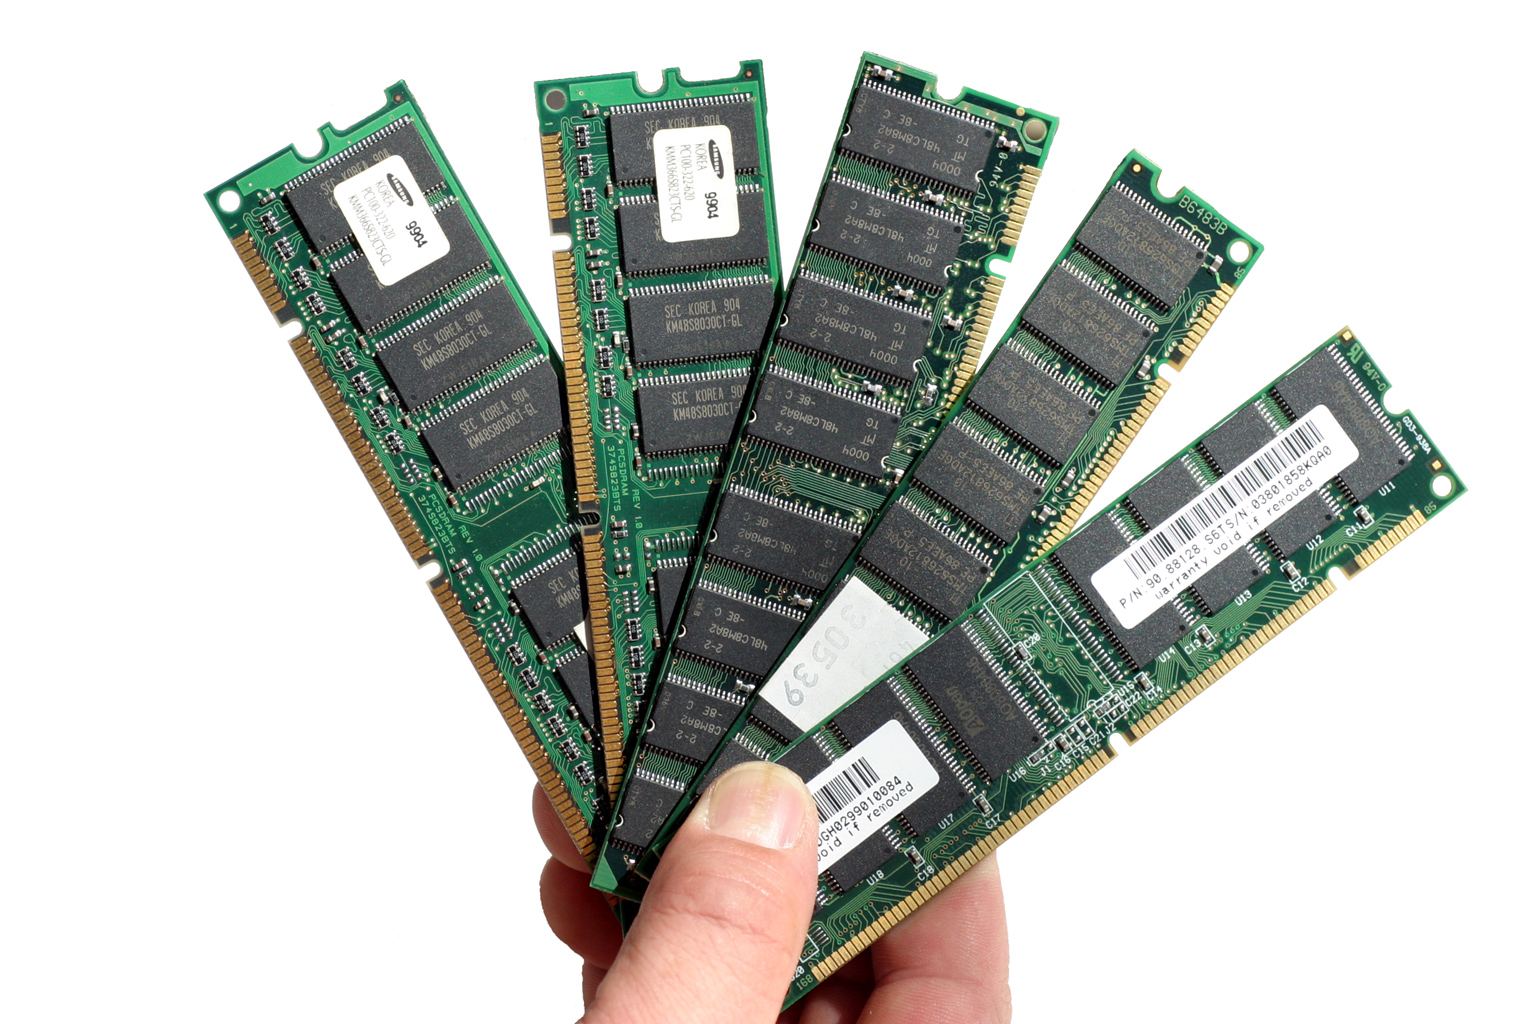
\includegraphics[width=10cm]{Memoria.jpg}
\centering
\caption{Memoria ram de un pc}
\label{fig:memoriapc}
\end{figure}
    
El paquete también agrega un comportamiento especial 
a <<estas marcas para hacer citas textuales>> tal como 
lo indican las reglas de la RAE.


A continuación se presenta el logo de C++ Figura 



En la sección de teoremas (\ref{contenido})

\section{Conclusión} \label{conclulsion}

\bibliographystyle{IEEEtran}
\bibliography{references}

\end{document}
